\titre{Question 1 b}
\begin{enumerate}
	\item Oui (voir contre exemple)
	\item Oui (voir contre exemple)
	\item Non pour un graphe connexe (le nombre d'arêtes d'un arbre dépend uniquement du nombre de noeud car chaque fois qu'on ajoute un noeud dans un arbre on ajoute une arête (sauf la racine))
\end{enumerate}

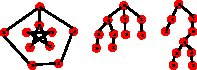
\includegraphics[width=300px]{Images/fig13.pdf}

\titre{Question 2}
\begin{enumerate}
	\item .\\ 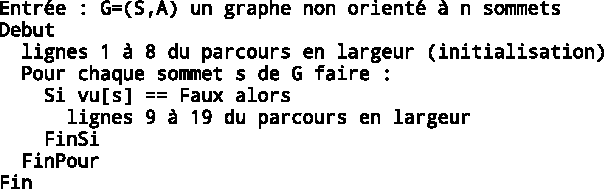
\includegraphics{Images/fig14.pdf}
	\item La forêt couvrante d'un graphe connexe est un arbre
\end{enumerate}

\titre{Question 3} Il suffit de rajouter un compteur dans l'algorithme précédent :\\
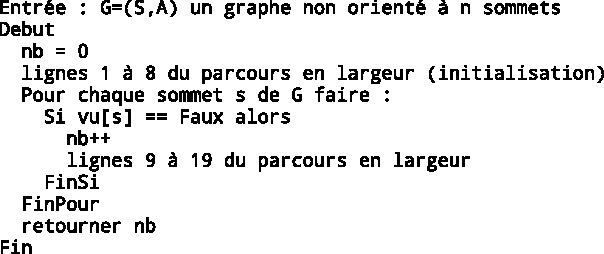
\includegraphics{Images/fig15.pdf}

\titre{Question 4} 
\begin{enumerate}
	\item .\\ 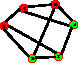
\includegraphics[width=100px]{Images/fig16.pdf}
	\item Un simple triangle n'est pas biparti
	\item On part du parcours en largeur ou en profondeur : on donne une couleur au premier voisin, puis l'autre à tous ces voisins qui n'ont pas de couleur, pour les autres voisins on regarde si ils sont de couleur différente, sinon on s'arrête en répondant non. \\ 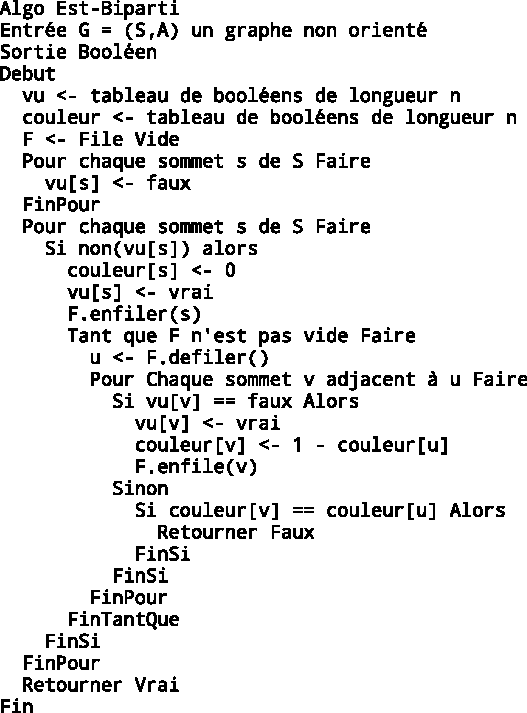
\includegraphics{Images/fig17.pdf}
\end{enumerate}

\titre{Question 5} \\ 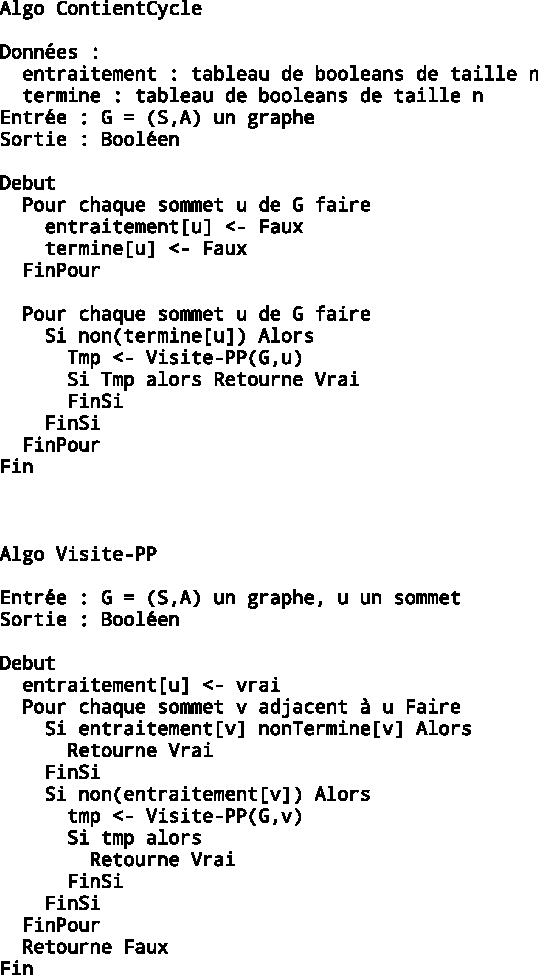
\includegraphics{Images/fig18.pdf}

